\documentclass[12pt,a4paper]{article}

% Margins.
\setlength{\oddsidemargin}{0in}
\setlength{\evensidemargin}{0in}
\setlength{\headheight}{12pt}
\setlength{\headsep}{42pt}
\setlength{\topmargin}{-54pt}
\setlength{\textwidth}{6.5in}
\setlength{\textheight}{10in}

\usepackage{amsmath}
\usepackage{float}
\usepackage{graphicx}
\usepackage[hyphens]{url}
\usepackage{hyperref}	% Clickable links to figures, references and urls.
\usepackage{datetime}
\usepackage{longtable}
\usepackage{subfigure}

% Links direct to top of figures.
\usepackage[all]{hypcap}

% Drawing.
\usepackage{pgf}
\usepackage{tikz}

% Listings for formatting code.
\usepackage{listings}
\usepackage{textcomp}
% General options.+++
\lstset{breaklines=true, basicstyle=\small\ttfamily, tabsize=4, numbers=left, stepnumber=1, frame=single, showstringspaces=false, upquote=true}
% C++ specific high-lighting. Comments are 50/50 shades of green/black and strings coloured with 60/40 red/black mixture.
\lstset{language=[ISO]C++, commentstyle=\color{green!50!black}, keywordstyle=\color{blue}, stringstyle=\color{red!60!black}}

%opening
\title{\vspace{-3cm}Physics for Engineers\\Class 30\\Magnetic Field}
\author{Attique Dawood}
\date{October 30, 2013\\[0.2cm] Last Modified: \today, \currenttime}
\begin{document}
\maketitle
\section{Announcements}
\begin{itemize}
\item None.
\end{itemize}
\section{Electric Flux Density}
In electrostatics a fundamental field quantity called electric flux density is related to electric field by the following relation
\begin{equation}
\textbf{D}=\epsilon\textbf{E}.
\end{equation}
Where
\begin{equation}
\epsilon=\epsilon_r\epsilon_0.
\end{equation}
For free space $\epsilon_r=1$. \textbf{D} has units Coulomb/m$^2$.
\section{Magnetic Field}
Magnetic field has the symbol \textbf{B} in physics and \textbf{H} in engineering. Engineering texts refer to \textbf{B} as magnetic flux density and vice versa. In principle we're going to refer to \textbf{H} as magnetic field and \textbf{B} as magnetic flux density but for the sake of consistency, when solving problems from Serway, we'll refer to \textbf{B} as magnetic field.

\textbf{H} has units Ampere/m and \textbf{B} has units Webers/m$^2$ or Tesla. Magnetic field and magnetic flux densities are related by
\begin{equation}
\textbf{B}=\mu\textbf{H}.
\end{equation}
Where $\mu$ is the permeability of the medium given by
\begin{equation}
\mu=\mu_r\mu_0.
\end{equation}
$\mu_r$ is the relative permeability and $\mu_0$ is the permeability of free space. For free space $\mu_r=1$. Since \textbf{H} and \textbf{B} are related by a constant we can pretty much refer to \textbf{B} as magnetic field for simplicity and consistency with physics text.
\section{Magnetic Force on a Charge in Motion}
Without going into details of sources of magnetic fields we consider the effect of magnetic field on charges in motion here. Presence of magnetic field can be detected with the help of magnetic compass. A compass will always align itself with the direction of magnetic field lines, for example, near a magnet.

If a magnetic field exists in a region then a charge moving in the magnetic field will experience a force due to magnetic field. This force is given by
\begin{equation}
\textbf{F}_B=q\textbf{v}\times\textbf{B}.
\end{equation}
Where \textbf{v} is the velocity of particle and \textbf{B} is magnetic flux density. The magnetic force acts perpendicular to the direction of motion and cannot change the speed of charge. It can, however, change the direction of motion. It is useful to define dot and cross notation for representing magnetic field as coming out of the page or going inside the page.
\section{Exercises}
\noindent\textbf{Question 1:} A 1 C charged particle moving with uniform velocity $\textbf{v}=3\hat y$ m/s enters a uniform magnetic field $\textbf{B}=10\hat z$ Wb/m$^2$. Calculate magnetic force on it.\\[0.2cm]
\noindent\textbf{Question 2:} An electron moves with uniform velocity $\textbf{v}=8\times 10^6\hat x$ m/s in a uniform magnetic field. If magnetic field of magnitude 0.025 Wb/m$^2$ is perpendicular to $z$--axis and makes an angle of $60^0$ with $x$--axis then find the force on electron.
%\begin{itemize}
%\item[a.] Electric field of a point charge.
%\item[b.] Electric field of an infinite line charge placed along $z$--axis.
%\end{itemize}
%%\begin{figure}[H]
%\centering
%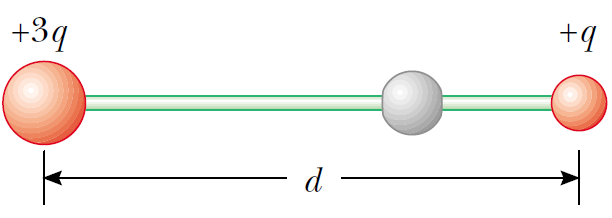
\includegraphics[scale=0.45]{FigureP23-10.png}
%\caption{Equilibrium of charge.}
%\label{Equilibrium}
%\end{figure}
%\nocite{*}
%\bibliographystyle{plain}
%\bibliography{PhysicsRef}
\end{document}
